\section{Understanding Buildroot internals}

\begin{frame}[fragile]{Configuration system}
  \begin{itemize}
  \item Uses, almost unchanged, the {\em kconfig} code from the
    kernel, in \code{support/kconfig} (variable \code{CONFIG})
  \item {\em kconfig} tools are built in
    \code{$(BUILD_DIR)/buildroot-config/}
  \item The main \code{Config.in} file, passed to *config, is at the
    top-level of the Buildroot source tree
  \end{itemize}
\begin{block}{}
\begin{minted}[fontsize=\tiny]{make}
CONFIG_CONFIG_IN = Config.in
CONFIG = support/kconfig
BR2_CONFIG = $(CONFIG_DIR)/.config

-include $(BR2_CONFIG)

$(BUILD_DIR)/buildroot-config/%onf:
        mkdir -p $(@D)/lxdialog
        ... $(MAKE) ... -C $(CONFIG) -f Makefile.br $(@F)

menuconfig: $(BUILD_DIR)/buildroot-config/mconf outputmakefile
        @$(COMMON_CONFIG_ENV) $< $(CONFIG_CONFIG_IN)
\end{minted}
\end{block}
\end{frame}

\begin{frame}{Configuration hierarchy}
  \begin{center}
    \includegraphics[width=\textwidth]{slides/buildroot-internals/config-hierarchy.pdf}
  \end{center}
\end{frame}

\begin{frame}{When you run {\tt make}...}
  \begin{center}
    \includegraphics[width=\textwidth]{slides/buildroot-internals/global-build-logic.pdf}
  \end{center}
\end{frame}

\begin{frame}[fragile]{Where is {\tt \$(TARGETS)} filled?}

\begin{block}{Part of \code{package/pkg-generic.mk}}
\begin{minted}[fontsize=\tiny]{make}

#  argument 1 is the lowercase package name
#  argument 2 is the uppercase package name, including a HOST_ prefix
#             for host packages

define inner-generic-package
 ...
$(2)_KCONFIG_VAR = BR2_PACKAGE_$(2)
 ...
ifeq ($$($$($(2)_KCONFIG_VAR)),y)
PACKAGES += $(1)
endif # $(2)_KCONFIG_VAR

endef # inner-generic-package
\end{minted}
\end{block}

\begin{itemize}
\item Adds the lowercase name of an enabled package as a make target
  to the \code{$(PACKAGES)} variable
\item \code{package/pkg-generic.mk} is really the core of the package
  infrastructure
\end{itemize}

\end{frame}

\begin{frame}{Diving into {\tt pkg-generic.mk}}

\begin{itemize}
\item The \code{package/pkg-generic.mk} file is divided in two main
  parts:
  \begin{enumerate}
  \item Definition of the actions done in each step of a package build
    process. Done through {\em stamp file targets}.
  \item Definition of the \code{inner-generic-package},
    \code{generic-package} and \code{host-generic-package} macros,
    that define the sequence of actions, as well as all the variables
    needed to handle the build of a package.
  \end{enumerate}
\end{itemize}

\end{frame}

\begin{frame}[fragile]{Definition of the actions: code}
  \begin{columns}
    \column{0.5\textwidth}
    \begin{block}{}
    \begin{minted}[fontsize=\tiny]{make}
$(BUILD_DIR)/%/.stamp_downloaded:
        # Do some stuff here
        $(Q)touch $@

$(BUILD_DIR)/%/.stamp_extracted:
        # Do some stuff here
        $(Q)touch $@

$(BUILD_DIR)/%/.stamp_patched:
        # Do some stuff here
        $(Q)touch $@

$(BUILD_DIR)/%/.stamp_configured:
        # Do some stuff here
        $(Q)touch $@

$(BUILD_DIR)/%/.stamp_built:
        # Do some stuff here
        $(Q)touch $@
      \end{minted}
      \end{block}
      \column{0.5\textwidth}
      \begin{block}{}
      \begin{minted}[fontsize=\tiny]{make}
$(BUILD_DIR)/%/.stamp_host_installed:
        # Do some stuff here
        $(Q)touch $@

$(BUILD_DIR)/%/.stamp_staging_installed:
        # Do some stuff here
        $(Q)touch $@

$(BUILD_DIR)/%/.stamp_images_installed:
        # Do some stuff here
        $(Q)touch $@

$(BUILD_DIR)/%/.stamp_target_installed:
        # Do some stuff here
        $(Q)touch $@
    \end{minted}
  \end{block}
 \end{columns}

 \begin{itemize}
 \item {\tt \$(BUILD\_DIR)/\%/} $\rightarrow$ build directory of any package
 \item a {\em make} target depending on one stamp file will trigger
   the corresponding action
 \item the {\em stamp file} prevents the action from being re-executed
 \end{itemize}

\end{frame}

\begin{frame}[fragile]{Action example 1: download}

\begin{block}{}
\begin{minted}[fontsize=\tiny]{make}
# Retrieve the archive
$(BUILD_DIR)/%/.stamp_downloaded:
        $(foreach hook,$($(PKG)_PRE_DOWNLOAD_HOOKS),$(call $(hook))$(sep))
        [...]
	$(foreach p,$($(PKG)_ALL_DOWNLOADS),$(call DOWNLOAD,$(p))$(sep))
        $(Q)mkdir -p $(@D)
        $(Q)touch $@
\end{minted}
\end{block}

\begin{itemize}
\item Step handled by the package infrastructure
\item In all {\em stamp file targets}, \code{PKG} is the upper case
  name of the package. So when used for Busybox,
  \code{$($(PKG)_SOURCE)} is the value of \code{BUSYBOX_SOURCE}.
\item {\em Hooks}: make macros called before and after each step.
\item \code{<pkg>_ALL_DOWNLOADS} lists all the files to be downloaded,
  which includes the ones listed in \code{<pkg>_SOURCE},
  \code{<pkg>_EXTRA_DOWNLOADS} and \code{<pkg>_PATCH}.
\end{itemize}

\end{frame}

\begin{frame}[fragile]{Action example 2: build}

\begin{block}{}
\begin{minted}[fontsize=\tiny]{make}
# Build
$(BUILD_DIR)/%/.stamp_built::
        @$(call step_start,build)
        @$(call MESSAGE,"Building")
        $(foreach hook,$($(PKG)_PRE_BUILD_HOOKS),$(call $(hook))$(sep))
        +$($(PKG)_BUILD_CMDS)
        $(foreach hook,$($(PKG)_POST_BUILD_HOOKS),$(call $(hook))$(sep))
        $(Q)touch $@
        @$(call step_end,build)
\end{minted}
\end{block}

\begin{itemize}
\item Step handled by the package, by defining a value for
  \code{<pkg>_BUILD_CMDS}.
\item Same principle of {\em hooks}
\item \code{step_start} and \code{step_end} are part of
  instrumentation to measure the duration of each step (and other
  actions)
\end{itemize}

\end{frame}

\begin{frame}[fragile]{The {\tt generic-package} macro}

\begin{itemize}
\item Packages built for the target:
\begin{block}{}
\begin{minted}[fontsize=\tiny]{make}
generic-package = $(call inner-generic-package,
                         $(pkgname),$(call UPPERCASE,$(pkgname)),
                         $(call UPPERCASE,$(pkgname)),target)
\end{minted}
\end{block}

\item Packages built for the host:
\begin{block}{}
\begin{minted}[fontsize=\tiny]{make}
host-generic-package = $(call inner-generic-package,
                              host-$(pkgname),$(call UPPERCASE,host-$(pkgname)),
                              $(call UPPERCASE,$(pkgname)),host)
\end{minted}
\end{block}

\item In \code{package/zlib/zlib.mk}:
\begin{block}{}
\begin{minted}[fontsize=\tiny]{make}
ZLIB_... = ...

$(eval $(generic-package))
$(eval $(host-generic-package))
\end{minted}
\end{block}

\item Leads to:
\begin{block}{}
\begin{minted}[fontsize=\tiny]{make}
$(call inner-generic-package,zlib,ZLIB,ZLIB,target)
$(call inner-generic-package,host-zlib,HOST_ZLIB,ZLIB,host)
\end{minted}
\end{block}

\end{itemize}

\end{frame}

\begin{frame}[fragile]{\code{inner-generic-package}: defining variables}

\begin{columns}

\column{0.5\textwidth}
\begin{block}{Macro code}
\begin{minted}[fontsize=\tiny]{make}
$(2)_TYPE    =  $(4)
$(2)_NAME    =  $(1)
$(2)_RAWNAME =  $$(patsubst host-%,%,$(1))

$(2)_BASE_NAME = $(1)-$$($(2)_VERSION)
$(2)_DIR       = $$(BUILD_DIR)/$$($(2)_BASE_NAME)



ifndef $(2)_SOURCE
 ifdef $(3)_SOURCE
  $(2)_SOURCE = $$($(3)_SOURCE)
 else
  $(2)_SOURCE ?=
    $$($(2)_RAWNAME)-$$($(2)_VERSION).tar.gz
 endif
endif

ifndef $(2)_SITE
 ifdef $(3)_SITE
  $(2)_SITE = $$($(3)_SITE)
 endif
endif

...
\end{minted}
\end{block}

\column{0.5\textwidth}
\begin{block}{Expanded for \code{host-zlib}}
\begin{minted}[fontsize=\tiny]{make}
HOST_ZLIB_TYPE    = host
HOST_ZLIB_NAME    = host-zlib
HOST_ZLIB_RAWNAME = zlib

HOST_ZLIB_BASE_NAME =
  host-zlib-$(HOST_ZLIB_VERSION)
HOST_ZLIB_DIR       =
  $(BUILD_DIR)/host-zlib-$(HOST_ZLIB_VERSION)

ifndef HOST_ZLIB_SOURCE
 ifdef ZLIB_SOURCE
  HOST_ZLIB_SOURCE = $(ZLIB_SOURCE)
 else
  HOST_ZLIB_SOURCE ?=
   zlib-$(HOST_ZLIB_VERSION).tar.gz
 endif
endif

ifndef HOST_ZLIB_SITE
 ifdef ZLIB_SITE
  HOST_ZLIB_SITE = $(ZLIB_SITE)
 endif
endif

...
\end{minted}
\end{block}

\end{columns}

\end{frame}

\begin{frame}[fragile]{\code{inner-generic-package}: dependencies}

\begin{block}{}
\begin{minted}[fontsize=\tiny]{make}
ifeq ($(4),target)
ifeq ($$($(2)_ADD_SKELETON_DEPENDENCY),YES)
$(2)_DEPENDENCIES += skeleton
endif
ifeq ($$($(2)_ADD_TOOLCHAIN_DEPENDENCY),YES)
$(2)_DEPENDENCIES += toolchain
endif
endif
\end{minted}
\end{block}

\begin{itemize}
\item Adding the \code{skeleton} and \code{toolchain} dependencies to
  target packages. Except for some specific packages (e.g. C library).
\end{itemize}
\end{frame}

\begin{frame}[fragile]{\code{inner-generic-package}: stamp files}

\begin{block}{}
\begin{minted}[fontsize=\tiny]{make}
$(2)_TARGET_INSTALL_TARGET =    $$($(2)_DIR)/.stamp_target_installed
$(2)_TARGET_INSTALL_STAGING =   $$($(2)_DIR)/.stamp_staging_installed
$(2)_TARGET_INSTALL_IMAGES =    $$($(2)_DIR)/.stamp_images_installed
$(2)_TARGET_INSTALL_HOST =      $$($(2)_DIR)/.stamp_host_installed
$(2)_TARGET_BUILD =             $$($(2)_DIR)/.stamp_built
$(2)_TARGET_CONFIGURE =         $$($(2)_DIR)/.stamp_configured
$(2)_TARGET_RSYNC =             $$($(2)_DIR)/.stamp_rsynced
$(2)_TARGET_RSYNC_SOURCE =      $$($(2)_DIR)/.stamp_rsync_sourced
$(2)_TARGET_PATCH =             $$($(2)_DIR)/.stamp_patched
$(2)_TARGET_EXTRACT =           $$($(2)_DIR)/.stamp_extracted
$(2)_TARGET_SOURCE =            $$($(2)_DIR)/.stamp_downloaded
$(2)_TARGET_DIRCLEAN =          $$($(2)_DIR)/.stamp_dircleaned
\end{minted}
\end{block}

\begin{itemize}
\item Defines shortcuts to reference the stamp files
\end{itemize}

\begin{block}{}
\begin{minted}[fontsize=\tiny]{make}
$$($(2)_TARGET_INSTALL_TARGET):         PKG=$(2)
$$($(2)_TARGET_INSTALL_STAGING):        PKG=$(2)
$$($(2)_TARGET_INSTALL_IMAGES):         PKG=$(2)
$$($(2)_TARGET_INSTALL_HOST):           PKG=$(2)
[...]
\end{minted}
\end{block}

\begin{itemize}
\item Pass variables to the stamp file targets, especially \code{PKG}
\end{itemize}

\end{frame}

\begin{frame}[fragile]{\code{inner-generic-package}: sequencing}

\begin{block}{Step sequencing for target packages}
\begin{minted}[fontsize=\tiny]{make}
$(1):                   $(1)-install

$(1)-install:           $(1)-install-staging $(1)-install-target $(1)-install-images

$(1)-install-target:            $$($(2)_TARGET_INSTALL_TARGET)
$$($(2)_TARGET_INSTALL_TARGET): $$($(2)_TARGET_BUILD)

$(1)-build:             $$($(2)_TARGET_BUILD)
$$($(2)_TARGET_BUILD):  $$($(2)_TARGET_CONFIGURE)

$(1)-configure:                 $$($(2)_TARGET_CONFIGURE)
$$($(2)_TARGET_CONFIGURE):      | $$($(2)_FINAL_DEPENDENCIES)
$$($(2)_TARGET_CONFIGURE):      $$($(2)_TARGET_PATCH)

$(1)-patch:             $$($(2)_TARGET_PATCH)
$$($(2)_TARGET_PATCH):  $$($(2)_TARGET_EXTRACT)

$(1)-extract:                   $$($(2)_TARGET_EXTRACT)
$$($(2)_TARGET_EXTRACT):        $$($(2)_TARGET_SOURCE)

$(1)-source:            $$($(2)_TARGET_SOURCE)

$$($(2)_TARGET_SOURCE): | dirs prepare
$$($(2)_TARGET_SOURCE): | dependencies
\end{minted}
\end{block}

\end{frame}

\begin{frame}{\code{inner-generic-package}: sequencing diagram}

\begin{center}
  \includegraphics[height=0.8\textheight]{slides/buildroot-internals/package-build-sequencing.pdf}
\end{center}

\end{frame}

\begin{frame}[fragile]{Example of package build}

\tiny
\begin{verbatim}
>>> zlib 1.2.8 Downloading
... here it wgets the tarball ...

>>> zlib 1.2.8 Extracting
xzcat /home/thomas/dl/zlib-1.2.8.tar.xz | tar ...

>>> zlib 1.2.8 Patching

>>> zlib 1.2.8 Configuring
(cd /home/thomas/projets/buildroot/output/build/zlib-1.2.8;
   ...
   ./configure --shared --prefix=/usr)

>>> zlib 1.2.8 Building
/usr/bin/make -j1 -C /home/thomas/projets/buildroot/output/build/zlib-1.2.8

>>> zlib 1.2.8 Installing to staging directory
/usr/bin/make -j1 -C /home/thomas/projets/buildroot/output/build/zlib-1.2.8
  DESTDIR=/home/thomas/projets/buildroot/output/host/arm-buildroot-linux-uclibcgnueabi/sysroot
  LDCONFIG=true install

>>> zlib 1.2.8 Installing to target
/usr/bin/make -j1 -C /home/thomas/projets/buildroot/output/build/zlib-1.2.8
  DESTDIR=/home/thomas/projets/buildroot/output/target
  LDCONFIG=true install
\end{verbatim}
\end{frame}

\begin{frame}[fragile]{Preparation work: dirs, prepare, dependencies}

  \begin{block}{pkg-generic.mk}
    \begin{minted}[fontsize=\tiny]{make}
$$($(2)_TARGET_SOURCE): | dirs prepare
$$($(2)_TARGET_SOURCE): | dependencies
    \end{minted}
  \end{block}

  \begin{itemize}
  \item All packages have three targets in their dependencies:
    \begin{itemize}
    \item \code{dirs}: creates the main directories (\code{BUILD_DIR},
      \code{TARGET_DIR}, \code{HOST_DIR}, etc.). As part of creating
      \code{TARGET_DIR}, the root filesystem skeleton is copied into
      it
    \item \code{prepare}: generates a kconfig-related \code{auto.conf}
      file
    \item \code{dependencies}: triggers the check of Buildroot system
      dependencies, i.e. things that must be installed on the machine
      to use Buildroot
    \end{itemize}
  \end{itemize}
\end{frame}

\begin{frame}[fragile]{Rebuilding packages?}
  \begin{itemize}
  \item Once one step of a package build process has been done, it is
    never done again due to the {\em stamp file}
  \item Even if the package configuration is changed, or the package
    is disabled $\rightarrow$ Buildroot doesn't try to be smart
  \item One can force rebuilding a package from its configure step or
    build step using \code{make <pkg>-reconfigure} or \code{make
      <pkg>-rebuild}
  \end{itemize}
  \begin{block}{}
    \begin{minted}[fontsize=\tiny]{make}
$(1)-clean-for-rebuild:
                        rm -f $$($(2)_TARGET_BUILD)
                        rm -f $$($(2)_TARGET_INSTALL_STAGING)
                        rm -f $$($(2)_TARGET_INSTALL_TARGET)
                        rm -f $$($(2)_TARGET_INSTALL_IMAGES)
                        rm -f $$($(2)_TARGET_INSTALL_HOST)

$(1)-rebuild:           $(1)-clean-for-rebuild $(1)

$(1)-clean-for-reconfigure: $(1)-clean-for-rebuild
                        rm -f $$($(2)_TARGET_CONFIGURE)

$(1)-reconfigure:       $(1)-clean-for-reconfigure $(1)
\end{minted}
\end{block}
\end{frame}

\begin{frame}{Specialized package infrastructures}
  \begin{itemize}
  \item The \code{generic-package} infrastructure is fine for packages
    having a {\bf custom} build system
  \item For packages using a {\bf well-known build system}, we want
    to factorize more logic
  \item Specialized {\bf package infrastructures} were created to
    handle these packages, and reduce the amount of duplication
  \item For {\em autotools}, {\em CMake}, {\em Python}, {\em Perl},
    {\em Lua} and {\em kconfig} packages
  \end{itemize}
\end{frame}

\begin{frame}[fragile]{CMake package example: {\tt flann}}

\begin{block}{package/flann/flann.mk}
\begin{minted}[fontsize=\tiny]{make}
FLANN_VERSION = d0c04f4d290ebc3aa9411a3322992d298e51f5aa
FLANN_SITE = $(call github,mariusmuja,flann,$(FLANN_VERSION))
FLANN_INSTALL_STAGING = YES
FLANN_LICENSE = BSD-3-Clause
FLANN_LICENSE_FILES = COPYING
FLANN_CONF_OPT = \
        -DBUILD_C_BINDINGS=ON \
        -DBUILD_PYTHON_BINDINGS=OFF \
        -DBUILD_MATLAB_BINDINGS=OFF \
        -DBUILD_EXAMPLES=$(if $(BR2_PACKAGE_FLANN_EXAMPLES),ON,OFF) \
        -DBUILD_TESTS=OFF \
        -DBUILD_DOC=OFF \
        -DUSE_OPENMP=$(if $(BR2_GCC_ENABLE_OPENMP),ON,OFF) \
        -DPYTHON_EXECUTABLE=OFF

$(eval $(cmake-package))
\end{minted}
\end{block}

\end{frame}

\begin{frame}[fragile]{CMake package infrastructure (1/2)}

\begin{block}{}
\begin{minted}[fontsize=\tiny]{make}
define inner-cmake-package

$(2)_CONF_ENV                   ?=
$(2)_CONF_OPT                   ?=
...

$(2)_SRCDIR                     = $$($(2)_DIR)/$$($(2)_SUBDIR)
$(2)_BUILDDIR                   = $$($(2)_SRCDIR)

ifndef $(2)_CONFIGURE_CMDS
ifeq ($(4),target)
define $(2)_CONFIGURE_CMDS
    (cd $$($$(PKG)_BUILDDIR) && \
     $$($$(PKG)_CONF_ENV) $$(HOST_DIR)/bin/cmake $$($$(PKG)_SRCDIR) \
         -DCMAKE_TOOLCHAIN_FILE="$$(HOST_DIR)/share/buildroot/toolchainfile.cmake" \
         ...
         $$($$(PKG)_CONF_OPT) \
    )
endef
else
define $(2)_CONFIGURE_CMDS
... host case ...
endef
endif
endif
\end{minted}
\end{block}

\end{frame}

\begin{frame}[fragile]{CMake package infrastructure (2/2)}

\begin{block}{}
\begin{minted}[fontsize=\tiny]{make}
$(2)_DEPENDENCIES += host-cmake

ifndef $(2)_BUILD_CMDS
ifeq ($(4),target)
define $(2)_BUILD_CMDS
        $$(TARGET_MAKE_ENV) $$($$(PKG)_MAKE_ENV) $$($$(PKG)_MAKE) $$($$(PKG)_MAKE_OPT)
            -C $$($$(PKG)_BUILDDIR)
endef
else
... host case ...
endif
endif

... other commands ...

ifndef $(2)_INSTALL_TARGET_CMDS
define $(2)_INSTALL_TARGET_CMDS
        $$(TARGET_MAKE_ENV) $$($$(PKG)_MAKE_ENV) $$($$(PKG)_MAKE) $$($$(PKG)_MAKE_OPT)
          $$($$(PKG)_INSTALL_TARGET_OPT) -C $$($$(PKG)_BUILDDIR)
endef
endif

$(call inner-generic-package,$(1),$(2),$(3),$(4))

endef

cmake-package = $(call inner-cmake-package,$(pkgname),...,target)
host-cmake-package = $(call inner-cmake-package,host-$(pkgname),...,host)
\end{minted}
\end{block}

\end{frame}

\begin{frame}[fragile]{Autoreconf in \code{pkg-autotools.mk}}
  \begin{itemize}
  \item Package infrastructures can also add additional capabilities
    controlled by variables in packages
  \item For example, with the \code{autotools-package} infra, one can
    do \code{FOOBAR_AUTORECONF = YES} in a package to trigger an {\em
      autoreconf} before the {\em configure} script is executed
  \item Implementation in \code{pkg-autotools.mk}
    \begin{block}{}
      \begin{minted}[fontsize=\tiny]{make}
define AUTORECONF_HOOK
        @$$(call MESSAGE,"Autoreconfiguring")
        $$(Q)cd $$($$(PKG)_SRCDIR) && $$($$(PKG)_AUTORECONF_ENV) $$(AUTORECONF)
             $$($$(PKG)_AUTORECONF_OPTS)
        ...
endef

ifeq ($$($(2)_AUTORECONF),YES)
...
$(2)_PRE_CONFIGURE_HOOKS += AUTORECONF_HOOK
$(2)_DEPENDENCIES += host-automake host-autoconf host-libtool
endif
      \end{minted}
    \end{block}
  \end{itemize}
\end{frame}

\begin{frame}{Toolchain support}
  \begin{itemize}
  \item One {\em virtual package}, \code{toolchain}, with two
    implementations in the form of two packages:
    \code{toolchain-buildroot} and \code{toolchain-external}
  \item \code{toolchain-buildroot} implements the {\bf internal
      toolchain back-end}, where Buildroot builds the cross-compilation
    toolchain from scratch. This package simply depends on
    \code{host-gcc-final} to trigger the entire build process
  \item \code{toolchain-external} implements the {\bf external
      toolchain back-end}, where Buildroot uses an existing pre-built
    toolchain
  \end{itemize}
\end{frame}

\begin{frame}{Internal toolchain back-end}

\begin{columns}
  \column{0.7\textwidth}
  \begin{itemize}
    \footnotesize
  \item Build starts with utility host tools and libraries needed for
    gcc (\code{host-m4}, \code{host-mpc}, \code{host-mpfr},
    \code{host-gmp}). Installed in
    \code{$(HOST_DIR)/{bin,include,lib}}
  \item Build goes on with the cross binutils, \code{host-binutils},
    installed in \code{$(HOST_DIR)/bin}
  \item Then the first stage compiler, \code{host-gcc-initial}
  \item We need the \code{linux-headers}, installed in
    \code{$(STAGING_DIR)/usr/include}
  \item We build the C library, \code{uclibc} in this example. Installed
    in \code{$(STAGING_DIR)/lib}, \code{$(STAGING_DIR)/usr/include}
    and of course \code{$(TARGET_DIR)/lib}
  \item We build the final compiler \code{host-gcc-final}, installed
    in \code{$(HOST_DIR)/bin}
  \end{itemize}
  \column{0.3\textwidth}
  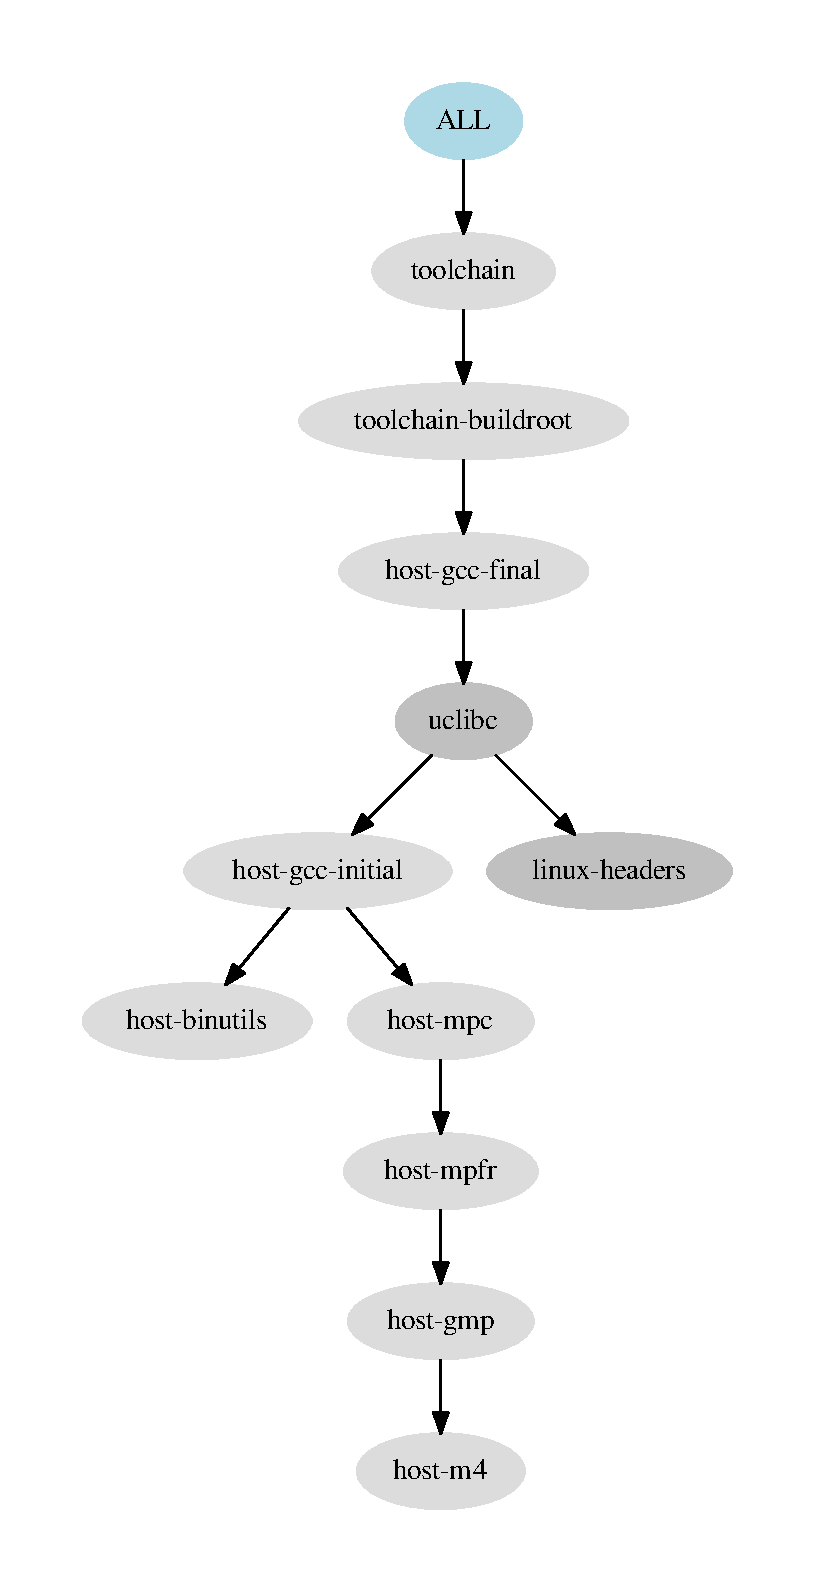
\includegraphics[width=\textwidth]{slides/buildroot-internals/internal-toolchain-graph-depends.pdf}
\end{columns}

\end{frame}

\begin{frame}{External toolchain back-end}
  \begin{itemize}
  \item Implemented as one package, \code{toolchain-external}
  \item Knows about well-known toolchains (CodeSourcery, Linaro, etc.)
    or allows to use existing custom toolchains (built with Buildroot,
    Crosstool-NG, etc.)
  \item Core logic:
    \begin{enumerate}
      \scriptsize
    \item Extract the toolchain to \code{$(HOST_DIR)/opt/ext-toolchain}
    \item Run some checks on the toolchain
    \item Copy the toolchain {\em sysroot} (C library and headers,
      kernel headers) to \code{$(STAGING_DIR)/usr/{include,lib}}
    \item Copy the toolchain libraries to \code{$(TARGET_DIR)/usr/lib}
    \item Create symbolic links or wrappers for the compiler, linker,
      debugger, etc from \code{$(HOST_DIR)/bin/<tuple>-<tool>} to
      \code{$(HOST_DIR)/opt/ext-toolchain/bin/<tuple>-<tool>}
    \item A wrapper program is used for certain tools (gcc, ld, g++,
      etc.) in order to ensure a certain number of compiler flags are
      used, especially \code{--sysroot=$(STAGING_DIR)} and
      target-specific flags.
    \end{enumerate}
  \end{itemize}
\end{frame}

\begin{frame}{Root filesystem image generation}
  \begin{itemize}
  \item Once all the targets in \code{$(PACKAGES)} have been built,
    it's time to create the root filesystem images
  \item First, the \code{target-finalize} target does some cleanup of
    \code{$(TARGET_DIR)} by removing documentation, headers, static
    libraries, etc.
  \item Then the root filesystem image targets listed in
    \code{$(ROOTFS_TARGETS)} are processed
  \item These targets are added by the common filesystem image
    generation infrastructure, in \code{fs/common.mk}
  \item The purpose of this infrastructure is to factorize the
    preparation logic, and then call {\em fakeroot} to create the
    filesystem image
  \end{itemize}
\end{frame}

\begin{frame}[fragile]{{\tt fs/common.mk}}
  \begin{block}{}
    \begin{minted}[fontsize=\tiny]{make}
define ROOTFS_TARGET_INTERNAL

ROOTFS_$(2)_DEPENDENCIES += host-fakeroot host-makedevs \
        $$(if $$(PACKAGES_USERS),host-mkpasswd)

$$(BINARIES_DIR)/rootfs.$(1): target-finalize $$(ROOTFS_$(2)_DEPENDENCIES)
        @$$(call MESSAGE,"Generating root filesystem image rootfs.$(1)")
        $$(foreach hook,$$(ROOTFS_$(2)_PRE_GEN_HOOKS),$$(call $$(hook))$$(sep))
        ...
        echo "chown -h -R 0:0 $$(TARGET_DIR)" >> $$(FAKEROOT_SCRIPT)
        echo "$$(HOST_DIR)/bin/makedevs -d $$(FULL_DEVICE_TABLE) $$(TARGET_DIR)" >> \
              $$(FAKEROOT_SCRIPT)
        echo "$$(ROOTFS_$(2)_CMD)" >> $$(FAKEROOT_SCRIPT)
        chmod a+x $$(FAKEROOT_SCRIPT)
        PATH=$$(BR_PATH) $$(HOST_DIR)/bin/fakeroot -- $$(FAKEROOT_SCRIPT)
        ...

rootfs-$(1): $$(BINARIES_DIR)/rootfs.$(1) $$(ROOTFS_$(2)_POST_TARGETS)

ifeq ($$(BR2_TARGET_ROOTFS_$(2)),y)
TARGETS_ROOTFS += rootfs-$(1)
endif
endef

define ROOTFS_TARGET
$(call ROOTFS_TARGET_INTERNAL,$(1),$(call UPPERCASE,$(1)))
endef
    \end{minted}
  \end{block}
\end{frame}

\begin{frame}[fragile]{{\tt fs/ubifs/ubifs.mk}}
  \begin{block}{}
    \begin{minted}[fontsize=\tiny]{make}
UBIFS_OPTS := -e $(BR2_TARGET_ROOTFS_UBIFS_LEBSIZE) \
              -c $(BR2_TARGET_ROOTFS_UBIFS_MAXLEBCNT) \
              -m $(BR2_TARGET_ROOTFS_UBIFS_MINIOSIZE)

ifeq ($(BR2_TARGET_ROOTFS_UBIFS_RT_ZLIB),y)
UBIFS_OPTS += -x zlib
endif
...

UBIFS_OPTS += $(call qstrip,$(BR2_TARGET_ROOTFS_UBIFS_OPTS))

ROOTFS_UBIFS_DEPENDENCIES = host-mtd

define ROOTFS_UBIFS_CMD
        $(HOST_DIR)/sbin/mkfs.ubifs -d $(TARGET_DIR) $(UBIFS_OPTS) -o $@
endef

$(eval $(call ROOTFS_TARGET,ubifs))
    \end{minted}
  \end{block}
\end{frame}

\begin{frame}{Final example}
  \begin{center}
    \includegraphics[width=\textwidth]{slides/buildroot-internals/final-example.pdf}
  \end{center}
\end{frame}
